% !TEX encoding = UTF-8 Unicode
% !TEX root = SystemTemplate.tex

\documentclass{book}

% !TEX root = SystemTemplate.tex

\usepackage[width=6.5in, height=9.2in, top=1.0in, papersize={8.5in,11in}]{geometry}
\usepackage[pdftex]{graphicx}
%\usepackage{draftwatermark}
\usepackage{amsmath}
\usepackage{amsthm}
\usepackage{amssymb}
%\usepackage{txfonts}
\usepackage{textcomp}
%\usepackage{amsthm}

\usepackage[all]{xy}
\usepackage{fancyhdr}
\pagestyle{fancy}
\usepackage{hyperref}
\usepackage{verbatim}
\usepackage{algorithm}
\usepackage{algorithmic}
\usepackage{array}
\usepackage{color}
\usepackage{listings}
\lstset{language=c,frame=ltrb,framesep=5pt,basicstyle=\normalsize,
 keywordstyle=\ttfamily\color{DarkRed},
identifierstyle=\ttfamily\color{DarkBlue}\bfseries,
commentstyle=\color{OliveGreen},
stringstyle=\ttfamily,
showstringspaces=false,tabsize = 3}
\usepackage{calc}
\usepackage{doxygen}
\usepackage[utf8]{inputenc}
\usepackage{makeidx}
\usepackage{multicol}
\usepackage{multirow}
\usepackage[table]{xcolor}
\usepackage{tabularx}
\usepackage{framed}
\usepackage{xspace}
\usepackage{etex}
\usepackage{todonotes}
\usepackage{pdfpages}
\usepackage{pgfgantt}


\definecolor{color02}{rgb}{0.18,0.35,0.59}
\definecolor{color03}{rgb}{0.44,0.59,0.82}
\definecolor{color06}{rgb}{0.35,0.35,0.35}


\newtheorem{summary}{Summary:}
\newtheorem{example}{Example:}


\definecolor{OliveGreen}{cmyk}{0.64,0,0.95,0.40}
\definecolor{DarkBlue}{cmyk}{0.76,0.76,0,0.20}
\definecolor{DarkRed}{cmyk}{0,1,1,0.45}


\def      \RR             {{\mathbb R}} 
\def      \DS            {\displaystyle} 

\setlength{\oddsidemargin}{0mm} 
\setlength{\evensidemargin}{0mm} 

%\SetWatermarkLightness{0.975}
%\SetWatermarkScale{6}
%\SetWatermarkText{\includegraphics{test.png}}

\pagestyle{fancy}
\renewcommand{\chaptermark}[1]{\markboth{#1}{}}
\renewcommand{\sectionmark}[1]{\markright{\thesection\ #1}}
\fancyhf{}
\fancyhead[LE,RO]{\bfseries\thepage}
\fancyhead[LO]{\bfseries\rightmark}
\fancyhead[RE]{\bfseries\leftmark}
%\fancyfoot[LE,RO]{Confidential and Proprietary}
%\renewcommand{\headrulewidth}{0.5pt}
%\renewcommand{\footrulewidth}{0pt}
%\addtolength{\headheight}{0.5pt}
%\setlength{\footskip}{0mm}
%\renewcommand{\footruleskip}{0pt}


\definecolor{MSBlue}{rgb}{.204,.353,.541}
\definecolor{MSLightBlue}{rgb}{.31,.506,.741}
\definecolor{MSBlue1}{rgb}{0.18,0.35,0.59}
\definecolor{MSBlue2}{rgb}{0.44,0.59,0.82}
\definecolor{MSBlue3}{rgb}{0.35,0.35,0.35}


\usepackage{titlesec}
\titleformat{\chapter}[display]
{\normalfont\bfseries\color{MSBlue1}}    %\normalfont\bfseries\filcenter}
{\LARGE\thechapter}
{1ex}
{\titlerule[2pt]
\vspace{2ex}%
\LARGE}
[\vspace{1ex}%
{\titlerule[2pt]}]

\definecolor{MSBlue}{rgb}{.204,.353,.541}
\definecolor{MSLightBlue}{rgb}{.31,.506,.741}
\definecolor{MSBlue1}{rgb}{0.18,0.35,0.59}
\definecolor{MSBlue2}{rgb}{0.44,0.59,0.82}
\definecolor{MSBlue3}{rgb}{0.35,0.35,0.35}

%\titleformat*{\section}{\Large\bfseries\sffamily\color{MSBlue}}
%\titleformat*{\subsection}{\large\bfseries\sffamily\color{MSLightBlue}}
%\titleformat*{\section}{\Large\bfseries\color{MSBlue1}}
%\titleformat*{\subsection}{\large\bfseries\color{MSBlue2}}

\titleformat*{\section}{\Large\bfseries\color{MSBlue}}
\titleformat*{\subsection}{\large\bfseries\color{MSLightBlue}}
\titleformat*{\subsubsection}{\large\bfseries\color{MSBlue3}}
\setcounter{secnumdepth}{3}
\renewcommand{\thesubsubsection}{\thesubsection.\alph{subsubsection}}

% Save the original chapter command as stdchapter
\let\stdchapter\chapter

%redefine the backmatter command
\let\stdbackmatter\backmatter
\makeatletter% We need the '@' letter to call if@openright
\renewcommand{\backmatter}{
\stdbackmatter
% need to set the page counter back to 1
\setcounter{page}{1}
%% Redefine the \chapter command for our Back Matter
\renewcommand{\chapter}[1]{
  \if@openright\cleardoublepage\else\clearpage\fi% chapters begin on right page
  \stdchapter{##1}% output standard chapter heading
  \setcounter{section}{0}% restart the section numbering
  \renewcommand{\thepage}{BM-\arabic{page}}% Redefine page numbering format
  \renewcommand{\thesection}{\arabic{section}}% Redefine section number format
}}
\makeatother% Restore the normal behavior of '@'

%redefine the appendix command
\let\stdappendix\appendix
\makeatletter% We need the '@' letter to call if@openright
\renewcommand{\appendix}{
\stdappendix
%% \titleformat{\chapter}[display]
%% {\normalfont\bfseries\color{MSBlue1}}    %\normalfont\bfseries\filcenter}
%% {\LARGE Appendix \thechapter}
%% {1ex}
%% {\titlerule[2pt]
%% \vspace{2ex}%
%% \LARGE}
%% [\vspace{1ex}%
%% {\titlerule[2pt]}]
  %%% Since counters are different in the appendix section
  %%% we redefine \chapter to explicitly reset the page number
  %%%  (comment out to see effect)
  \renewcommand{\chapter}[1]{
    \stdchapter{##1}\setcounter{page}{1}
    %%% We also redefine page numbering
    \renewcommand{\thepage}{\Alph{chapter}-\arabic{page}}
  }
}
\makeatother% Restore the normal behavior of '@'


\makeatletter% We need the '@' letter to call if@openright
\newcommand{\agreement}{
  \renewcommand{\chapter}[1]{
    \if@openright\cleardoublepage\else\clearpage\fi% chapters begin on right page
    \pagestyle{plain}% turn off fancy headers
    \setcounter{section}{0}% Reset the section number
    \setcounter{page}{1}% Reset the page number
    \renewcommand{\thepage}{SA-\arabic{page}}% Set format for page numbering
    \renewcommand{\thesection}{\arabic{section}}% Set format for section numbering
    \refstepcounter{chapter}% Add it to the index/toc for on-line viewing
    \addcontentsline{toc}{chapter}{##1}% Add to the table of contents
  }
}
\makeatother% Restore the normal behavior of '@'


 % This sets the format.

% Add your title page contents here 
\title{{\color{MSBlue1} \rule{\linewidth}{0.5mm}}\\[2mm] {\huge \bfseries \color{MSBlue1} Moonrockers}\\[-1mm] {\color{MSBlue1}\rule{\linewidth}{0.5mm}} \\  \vfill
{\LARGE \bfseries \color{MSBlue2} Senior Design Final Documentation }\\  \vfill 
{\color{MSBlue1} Moonrockers} }
\author{\color{MSBlue1}  Alexander Muchow}
\date{\color{MSBlue1} \today}


\begin{document}

\frontmatter

\addcontentsline{toc}{chapter}{Title}
\maketitle
\tableofcontents
\addcontentsline{toc}{chapter}{Contents}
\listoffigures
\addcontentsline{toc}{chapter}{List of Figures}
\listoftables
\addcontentsline{toc}{chapter}{List of Tables}
\listofalgorithms
\addcontentsline{toc}{chapter}{List of Algorithms}

\chapter{Overview Statements}
% !TEX root = SystemTemplate.tex

\section{Mission Statement}
The mission of this team is to implement software into the Moonrockers robot, both telelcommunications and autonomous. We plan to implement computer vision based algorithms to determine location based a image at a fixed point. From there, we will begin to implement the autonomy algorithms in which the robot will complete the tasks of our competition. 

  % add mission statement to mission.tex

\chapter{Document Preparation and Updates}
% !TEX root = SystemTemplate.tex



Current Version [1.3.0]
\vspace*{5mm}

{\color{MSBlue3}
\noindent
\textit{Prepared By:}\\
\textit{Alexander Muchow}\\
}

\vfill
\noindent
{\color{color02} \textit{\textbf{Revision History}}}\\
\begin{tabular}{|>{\raggedright}p{1.5cm}|>{\raggedright}p{3cm}|>{\raggedright}p{1.5cm}|>{\raggedright}p{9cm}|}
\hline
\textit{\textbf{Date}} &  \textit{\textbf{Author}} & \textit{\textbf{Version}} & \textit{\textbf{Comments}}\tabularnewline
\hline
 \textit{\textbf{09/21/15}} & \textit{Alexander Muchow} & \textit{1.0.0} & \textit{Initial version}\tabularnewline
\hline
\textit{\textbf{10/08/15}} & \textit{Alexander Muchow} & \textit{1.1.0} & \textit{Added in Sprint 1 Report }\tabularnewline
\hline
\textit{\textbf{11/05/15}} & \textit{Alexander Muchow} & \textit{1.2.0} & \textit{Added in Sprint 2 Report }\tabularnewline
\hline
\textit{\textbf{12/04/15}} & \textit{Alexander Muchow} & \textit{1.3.0} & \textit{Added in Sprint 3 Report }\tabularnewline
\hline
 &  &  & \tabularnewline
 \hline
 &  &  & \tabularnewline
\hline
 &  &  & \tabularnewline
\hline
 &  &  & \tabularnewline
\hline
 &  &  & \tabularnewline
\hline
\end{tabular}
\vfill


 
\mainmatter

%%  Add to the following chapters

% !TEX root = SystemTemplate.tex

\chapter{Overview and concept of operations}

The overview should take the form of an executive summary.  Give the reader a feel 
for the purpose of the document, what is contained in the document, and an idea 
of the purpose for the system or product. 


\section{Scope}
This document will cover the methods of development, as well as algorithms and systems, of the moonrockers team. It will discuss the major components we will be developing, as well as their roles.

\section{Deliverables}

The client has requested improvements to their telecommunication code, as well as to begin working on the autonomy portion of the robot.

\section{Purpose}
The purpose of this system is to be able to control the robot which the team has build. The robot's goal is to go and mine regolith, in order to return it to a collection bin. The team would prefer to do this autonomously as it would gain a significant amount of additional points in the competition.


\subsection{Vision based location}
This component will playa major role in this system because it will determine where the robot is located within the competition pit. We plan to do this via attaching an AR tag to the collection bin in which we deposit our material, and then mount one or more cameras onto our robot. The cameras will use an algorithm to determine the distance and orientation in which they are located relative to the AR tag. This is important, as we are driving on a sandlike material, and typical odometry will not be nearly as effective as this vision based system.

\subsection{Location based Decision Making}
This will allow us to make decisions based on where we are within the competition pit, for instance is we are too close to a certain wall, we will turn away from it, or if we are to the mining portion of the pit, we will begin mining. The first component is very important for this one because we will need to be able to tell where we are relative to the collection bin in order to do this.
\newpage
\subsection{Telecommunication}
This is another very important part of the robot's system, as it allows a user to directly control the robot. There is currently software in place for this, but it requires many improvements and also the ability to override the autonomous system if the need were to arise.

\section{Systems Goals}
The goals for this system to acheive are being able to perform in the competition pit autonomously to acheive some of the points available, as well as be able to receive points for mining material.

\section{System Overview and Diagram}
The major system components will interact in the manner seen in the diagram below. As you can see, our ODroid XU4 is running ROS, which will support both the Vision based location node and the decision making portion of the system. It will pass messages from the vision based location system to the decision making system, and then that will tell the Odroid what to tell the PCDuino to tell the robot. 

At the same time, you can see the manual control via a windows PC . Currently the windows PC and the PCDuino connect to the same network and then form a TCP server to transmit information from the controller to the robot.


\begin{figure}[tbh]
\begin{center}
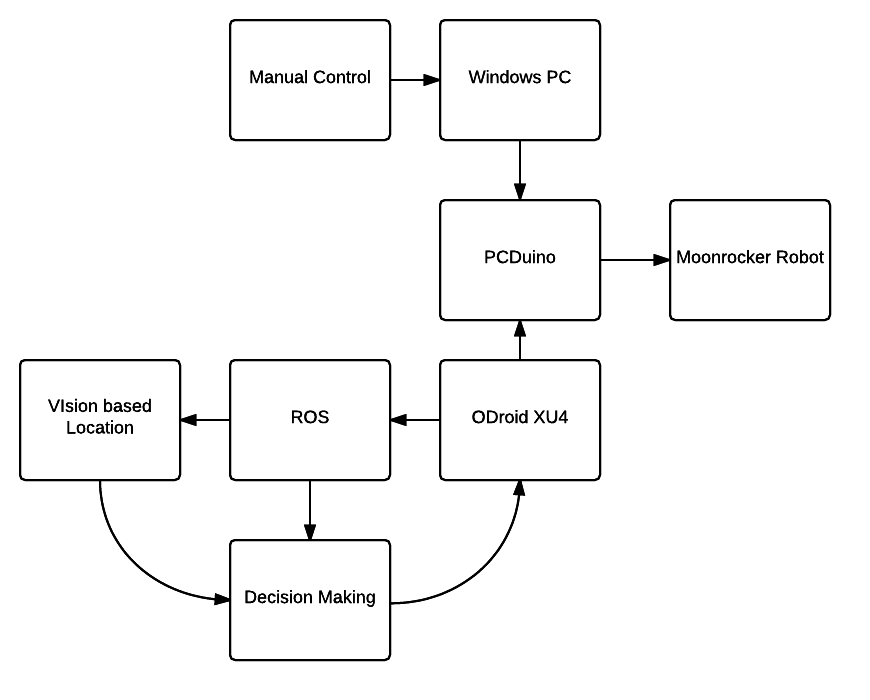
\includegraphics[width=0.75\textwidth]{./design}
\end{center}
\caption{System Diagram \label{systemdiagram}}
\end{figure}
\newpage
\section{Technologies Overview}
The technologies used to develop this system are the PCDuino, ODroid XU4, and ROS.
\vspace{2mm}

We chose to use the ODroid XU4 because it has 2 quad core processors which will be able to sufficiently handle the vision system, as well as the decision making system.
\vspace{2mm}


We chose to use ROS because it will help integrate the sensors in our system with the controls.
\vspace{2mm}


We chose to use the PCDuino because it was already integrated into our robotics system from the last year and currently runs out manual control systems.



  %% All tracks
% !TEX root = SystemTemplate.tex


\chapter{Project Overview}







\section{Team Members and Roles}
\hspace{5 mm}\underline{Autonomy}


Alex Muchow, Computer Science


Devin Kroeber, Electrical Engineering
\vspace{5 mm}


\underline{Moonrockers System}


Daniel Hodges, Mechanical Engineering

q
Samiel Hill, Mechanical Engineering


Jacob Green, Mechanical Engineering

\vspace{5 mm}
\underline{Icy Regolith}


Erik Figuracion, Mechanical Engineering


Mathew Gordon, Mechanical Engineering


Jonathan Stelzle, Mechanical Engineering



\section{Project  Management Approach}
For this project we will be managing through the Agile methodology. The length of each sprint will be two weeks long, and there will be a week in between for review and a report. The product backlog is currently in trello, but as there has been a lot of overhead work, the backlog remains as it originally stood. Trello will be used to update progress on each backlog item, and to address items being done during each sprint., as well as bug tickets.

\section{Phase  Overview}

	\vspace{\baselineskip}
	\textbf{Phase 1: 0.1}

	\begin{itemize}
	\item AR Tag designed
	\item ASUS Xtion location relative to AR tag
	\item Find a location to mount the camera sensor on the robot.
	\end{itemize}


	\vspace{\baselineskip}
	\vspace{\baselineskip}
	\vspace{\baselineskip}
	
	\newpage
	\textbf{Phase 2: 0.5}

	\begin{itemize}
	\item Robot able to center itself at the AR tag from any start location and orientation
	\item Find a way to mount the AR tag at the dump station
	\end{itemize}
	

	\vspace{\baselineskip}
	\textbf{Phase 3: 1.0}

	\begin{itemize}
	\item Robot successfully able to travel the distance from the dump station, over the obstacle course to the mining site, and travel back.
	\item Robot able to perform a mining routing
	\item Robot able to performing dumping at the AR tagged dumping station after navigating back
	\end{itemize}
	
	\vspace{\baselineskip}
	\textbf{Phase 4: 1.1}
	
	\begin{itemize}
	\item Manual override

	
	\end{itemize}
	\vspace{\baselineskip}


\section{Terminology and Acronyms}
\hspace{ 5mm}Regolith - Black Point-1(BP-1), or simulant for mars soil.

Icy Regolith - Simulant for larger pieces of martian soil, in our competition it is gravel.


NRMC - NASA Robotic Mining Competition.


ROS - Robot Operating System
   %% All tracks
% !TEX root = SystemTemplate.tex
\chapter{User Stories,  Requirements,Backlog and Deliverables}
\section{Overview}
This section of the report will contain all of my user stories and discuss the entirety of the backlog and requirements


\subsection{Scope}

This portion will cover each user story in depth. The tests for each of those stories will be covered in the testing section of the design document.



\subsection{Purpose of the System}
The purpose of this system is to autonomously run the Moonrockers robot at the NRMC.


\section{ Stakeholder Information}

The stakeholders in this competition are myself and the moonrockers team.

This section would provide the basic description of all of the stakeholders for 
the project.  Who has an interest in the successful and/or unsuccessful completion 
of this project? 


\subsection{Customer or End User (Product Owner)}
The Product Owner is the moonrockers team. They will oversee the product and prioritize things in the backlog. They will interact with me throughout the project to drive it forward.

\subsection{Management or Instructor (Scrum Master)}
There will be no scrum master in this project.



\subsection{Developers --Testers}
I will be the one testing, designing, and developing.


\section{Requirements and Design Constraints}
The requirements for this project is that I develop and autonomous system to control the robot during the competition. The robot needs to navigate from its starting position, over the obstacle section, to the mining section of the pit. From there it needs to mine in the pit, and then backtrack through the obstacle section and deposit what it has mined in the collection bin, and repeat for the entire 10 minute run.  As far as 

\subsection{System  Requirements}

The system must run on and ODroid and fit inside of the current electronics box.


\subsection{Network Requirements}
We currently use a router to transmit data from one device to another.


\subsection{Development Environment Requirements}
Must run in Ubuntu 14.04


\subsection{Project  Management Methodology}
There will be two meetings a week. One with the advisors, and one with the remainder of the team. We will discuss the backlog during each meeting and also discuss progress made. There will be a total of six sprints throughout this project and the team will have access to the sprint and product backlogs if desired. Each sprint will last two weeks and there will be a review week after each sprint. There are no restrictions on source control as it will be hosted on github and only have one developer committing to the repository.

\section{User Stories}


\subsection{User Story \#1}
As a robot, I want to be autonomous.

\subsubsection{User Story \#1 Breakdown}
The project as a whole requires the robot to be autonomous, and will perform various tasks in the competition pit.

\subsection{User Story \#2} 
As a robot, I want to be able to see the collection bin and determine my location from it.

\subsubsection{User Story \#2 Breakdown}
We will need to base our location off of an AR tag attached that will be attached to the collection bin. We have received code from Daniel Nix from his project he did last year in senior design. We will be using this code to implement our vision system.

\subsection{User Story \#3} 
As a robot, I want to be able to navigate to a predefined location within the competition pi
\subsubsection{User Story \#3 Breakdown}
We will need to be able to navigate to predefined locations, as we we will need to move from the starting location to the mining section. This will require knowing where we are in the pit.

\subsection{User Story \#4} 
As a robot I want to mine in a predefined area.
\subsubsection{User Story \#4 Breakdown}
Once the robot reaches a certain area, it will need to begin mining. This will require sending a signal to the robot to begin mining once it reaches that area.


\subsection{User Story \#5} 
As a robot, I want to return to the collector bin and deposit what i've mined.
\subsubsection{User Story \#5 Breakdown}
The robot will need to return over the obstacle section to the collector bin and dump what it has mined. This will use the previous user story and expand on it by backing up to the collector bin and then activating the dump routine.



\section{Research Results}
Up to this point a lot was researched for the robot. It was decided to use an ODroid XU4 for the processing, as well as use ROS for programming the system.

  %% Not research track
% !TEX root = SystemTemplate.tex

\chapter{Design  and Implementation}
This section will go over all of the design and implementation details of the system. There are three main components to our project. They are the vision system, the decision making system, and the telecommunication system.

The vision system will allow the robot to be able to tell where it is within the competition pit. This is necessary due to the terrain being very sandy, thus causing typicaly methods of odometry to be uneffective.

The decision making system will allow the robot to make decisions when in the competition pit. This will be the brain of the robot and will tell all of the working parts what to do. We will have various logic setup for all of the areas of the pit, as well as data being stored as to wether or not it has been mining for a long enough to take its collected material back to dump, if it's stuck.

\section{Vision based location }

\subsection{Technologies  Used}
For this component, we will be using a rgb camera, as well as an ODroid XU4, and it will be supported by ROS. We will be mounting the camera on the back of the robot, and this will allow us to back up to the collection bin with precision. We are also using an AR tag that will be attached to the collector bin.

\subsection{Component  Overview}
As far as features of this component goes, it will allow a user, the robot in this case, to point a camera at the AR tag and be able to know how far away it is, and what angle you are viewing it from.

\subsection{Phase Overview}
This is an extension of the Phase Overview above, but specific to this component. 
 It is meant to be basically a brief list with space for marking the phase status. 


\subsection{Design Details}
Will be documented once code is up and running.


\section{Decision making system}

\subsection{Technologies  Used}
This component will use the visual location component, and then also be running on the ODroid XU4 via ROS. 


\subsection{Component  Overview}
The features of this system will include:
\itemize
\item{Ability to navigate from the starting location to the mining area}
\item{The ability to mine in the mining area after determining that it is in the mining area}
\item{The ability to back up to the collector bin after mining}
\item{The ability to get the robot unstuck if it has not moved within a certain amount of time}
\item{The ability to not run into walls}
\enditemize


\subsection{Design Details}
Will be further documented after vision system is implemented.


\section{Telecommunication }

\subsection{Technologies  Used}
This component uses a computer running windows, a router, an xbox controller, and a PCDuino. 

\subsection{Component  Overview}
The features of the telecommunication system is mainly just controlling the robot from the xbox controller.

\subsection{Data Flow Diagram}

\begin{figure}[tbh]
\begin{center}
\includegraphics[width=0.75\textwidth]{./telecomm}
\end{center}
\caption{System Diagram \label{systemdiagram}}
\end{figure}

\subsection{Design Details}
Currently, this system is working by interacting the windows pc with the pcduino via a TCP server set up on the network that they are both connected to. The windows program repeatedly loops and takes in the xbox controllers input and then sends over an array to the PCDuino, which maps each array variable to a pin which is connected to a working part of the robot. We currently have our drive motors mapped to the control sticks on the robot, as well as forward and reverse for our conveyor system mapped to the Y and Right Bumper buttons, and the dumping mechanism mapped to the Left Bumper and B buttons.


  %% All tracks
% !TEX root = SystemTemplate.tex

\chapter{System  and Unit Testing}

This section describes the approach taken with regard to system and unit testing. 

\section{Overview}
For a lot of our testing, we will be performing live tests on the robot once the code is on there. We will be testing on the replica collection bin that we have in our lab during the winter, and then we will be testing out on the sand volleyball court once the weather gets nicer. 



\section{Test Setup and Execution}


\subsection{Test \#1}
As a robot, I want to be autonomous.

\subsubsection{Test \#1 Breakdown}
We will be setting up a simulated competition pit in the sand volleyball court once each individual section has been tested.

\subsection{Test \#2} 
As a robot, I want to be able to see the collection bin and determine my location from it.

\subsubsection{Test \#2 Breakdown}
We will be walking the camera around our lab and testing the vision algorithms to be sure they are functioning properly.

\subsection{Test \#3} 
As a robot, I want to be able to navigate to a predefined location within the competition pit
\subsubsection{Test \#3 Breakdown}
We will be running the robot around the lab and setting up locations where it will travel from and to.

\subsection{Test \#4} 
As a robot I want to mine in a predefined area.
\subsubsection{Test \#4 Breakdown}
We will be using the previous test to take us to a location and then make sure it will mine once it gets there.


\subsection{Test \#5} 
As a robot, I want to return to the collector bin and deposit what i've mined.
\subsubsection{Test \#5 Breakdown}
We will be starting the robot at some distance from the collector bin, and then having it travel back to the collector bin, orient itself to be facing away from it, back up, and then dump into the collector bin.

  %% All tracks
% !TEX root = SystemTemplate.tex
\chapter{Development Environment}


\section{Development IDE and Tools}
There were no IDE's used for this project, we only used vim to do the file editing in ubuntu.

\section{Source  Control}
For this project, we used git via github for source control. We set it up on our ODroid and our PCDuino and have two repository's, one for telecommunication and one for autonomy. A developer connects to it by pulling down the repository and loggin in via their credentials that have access to the repository. 

\section{Dependencies}
\hspace{ 5mm}ROS Indigo


ODroid XU4 running Ubuntu 14.04

\section{Build  Environment}
There will be build scripts once we are in that stage of the project.
 %% All tracks
% !TEX root = SystemTemplate.tex

\chapter{Release -- Setup -- Deployment}
Will be placed in document second semester
%This section should contain any specific subsection regarding specifics in releasing, 
%setup, and/or deployment of the system. 


\section{Deployment Information and Dependencies}
%Are there dependencies that are not embedded into the system install? 



\section{Setup Information}
%How is a setup/install built? 



\section{System  Versioning Information}
%How is the system versioned? 
  %% Normally not research track
% !TEX root = SystemTemplate.tex

\chapter{User Documentation}
 Will be placed in document second semester
%This section should contain the basis for any end user documentation for the system. 
% End user documentation would cover the basic steps for setup and use of the system. 
 %It is likely that the majority of this section would be present in its own document 
%to be delivered to the end user.  However, it is recommended the original is contained 
%and maintained in this document. 

%\newpage   %% 
%%  The user guide can be an external document which is included here if necessary ...
%%  a single source is the way to go.

\section{User Guide}

%The source for the user guide can go here.    You have some options for how to handle the user docs.  If you have some {\tt newpage} commands around the guide then you can just print out those pages.   If a different formatting is required, then have the source in a separate file {\tt userguide.tex} and include that file here.  That file can also be included into a driver (like the senior design template) which has the client specified formatting.  Again, this is a single source approach.   


%% \newpage  %%  if needed ...
\section{Installation Guide}


%% \newpage  %%  if needed ...
\section{Programmer Manual}

 %% All tracks
% !TEX root = SystemTemplate.tex

\chapter{Class Index}
\section{Class List}
Here are the classes, structs, unions and interfaces with brief descriptions

\chapter{Class Documentation}

Will be discussed as the software is further developed
  %% All tracks

%\bibliographystyle{plain}
%\bibliography{designrefs.bib}
%\addcontentsline{toc}{chapter}{Bibliography}


% We want to add the Software agreement to the end and number the
% pages separately from the document.  We don't want to do a standard
% chapter heading, but we do want it to appear in the table of contents
% and in the index used for on-line viewing.  We defined the \agreement
% macro to set things up for us.
\agreement

\chapter{Software Agreement}
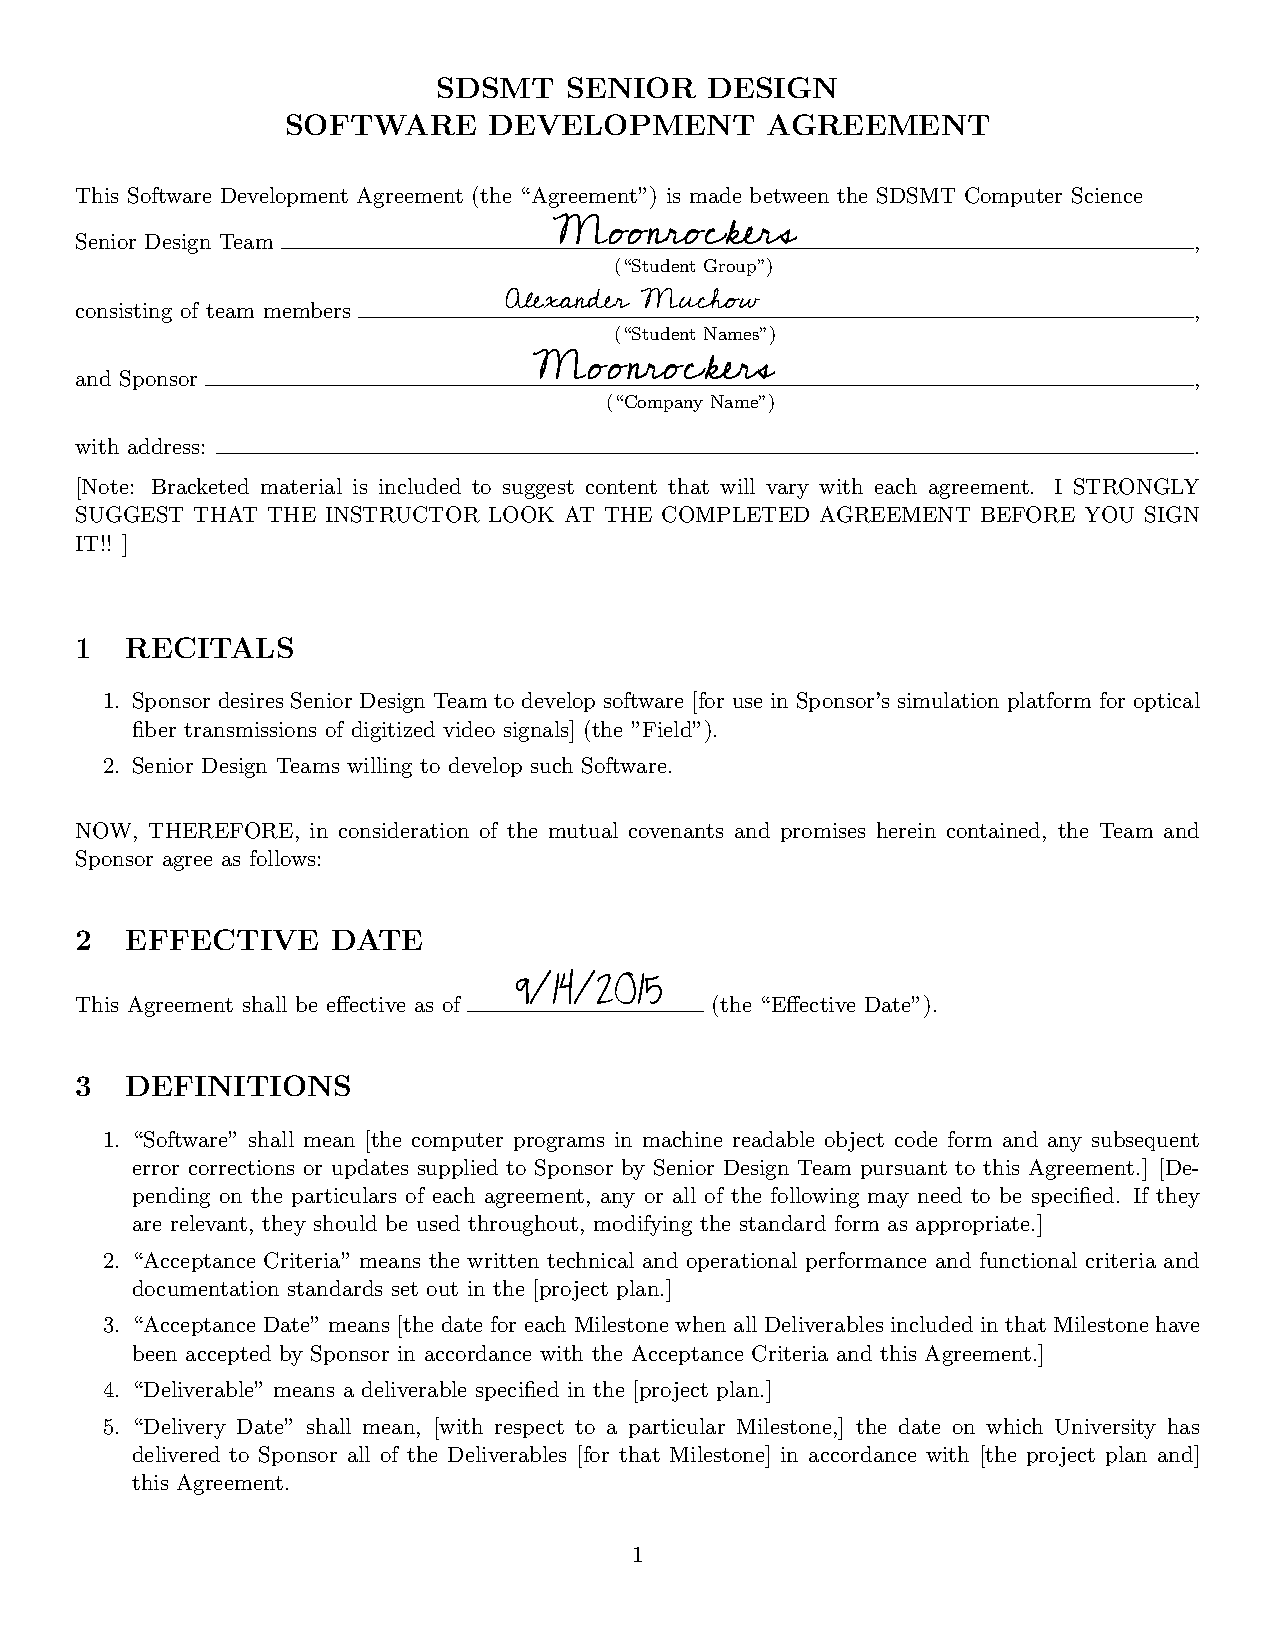
\includepdf[pages={1-5}]{SoftwareContract.pdf}

% In our style file, appendices are numbered with capital letters
\appendix

\chapter{Product Description}


Write a description of the product to be developed.
Use sectioning commands as neccessary.
\vspace{2\baselineskip}

\centerline{\Large {\bf NOTE:} {\em This is part of the contract.}}




\chapter{Sprint Reports}
% !TEX root = SystemTemplate.tex


\section{Sprint Report \#1}
\includepdf{sprint1.pdf}

\section{Sprint Report \#2}
\includepdf{sprint2.pdf}
\section{Sprint Report \#3}
\includepdf{sprint3.pdf}



\chapter{Industrial Experience and Resumes}
% !TEX root = SystemTemplate.tex


\section{Resumes}

\subsection{Alex Muchow}


\includepdf{MuchowResume.pdf}







\chapter{Acknowledgment}
\label{SpecialThanks}  
Thanks  

\chapter{Supporting Materials}

This document will contain several appendices used as a way to separate out major 
component details, logic details, or tables of information.  Use of this structure 
will help keep the document clean, readable, and organized. 



% chapters in backmatter don't have numbers, but they appear in the
% table of contents, and are numbered BM-X where X is the page number
% relative to where the backmatter begins.
\backmatter

%% Example
%\chapter{Course Syllabus}
%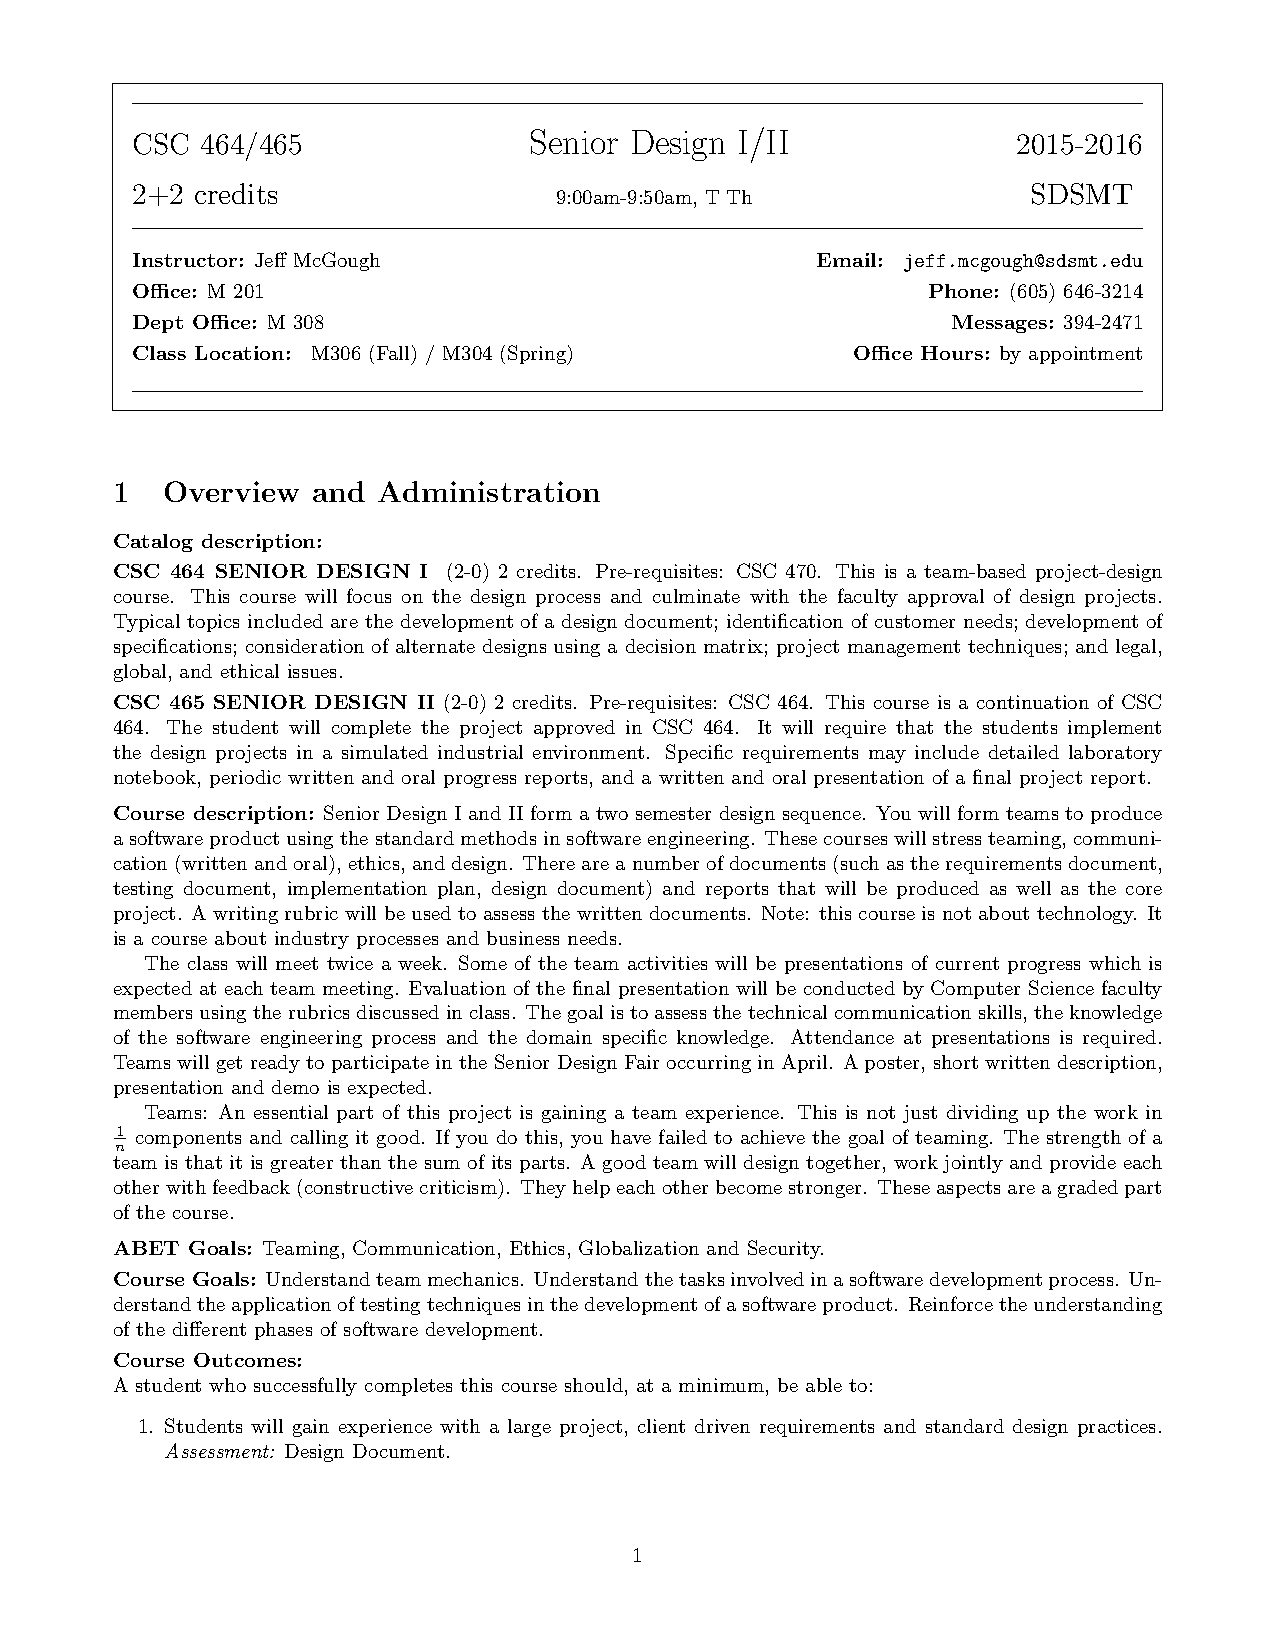
\includepdf[pages={1-17}]{syllabus.pdf}




\end{document}
